\documentclass[journal,comsoc]{IEEEtran}
\usepackage[portugues,ruled]{algorithm2e}
\usepackage{algorithmic}

\usepackage[T1]{fontenc}% optional T1 font encoding

\ifCLASSINFOpdf
\else
\fi
\usepackage[table]{xcolor}

\usepackage{color}
\usepackage{graphicx}
\usepackage{amsmath}
\interdisplaylinepenalty=2500
\usepackage[cmintegrals]{newtxmath}

\hyphenation{op-tical net-works semi-conduc-tor}

\begin{document}

\title{[Draft]Less capacity algorithm}

\author{Michael~Shell,~\IEEEmembership{Member,~IEEE,}
        John~Doe,~\IEEEmembership{Fellow,~OSA,}
        and~Jane~Doe,~\IEEEmembership{Life~Fellow,~IEEE}% <-this % stops a space
\thanks{M. Shell was with the Department
of Electrical and Computer Engineering, Georgia Institute of Technology, Atlanta,
GA, 30332 USA e-mail: (see http://www.michaelshell.org/contact.html).}% <-this % stops a space
\thanks{J. Doe and J. Doe are with Anonymous University.}% <-this % stops a space
\thanks{Manuscript received April 19, 2005; revised August 26, 2015.}}

\markboth{Journal of \LaTeX\ Class Files,~Vol.~14, No.~8, August~2015}%
{Shell \MakeLowercase{\textit{et al.}}: Bare Demo of IEEEtran.cls for IEEE Communications Society Journals}

\maketitle

\begin{abstract}
The abstract goes here.
\end{abstract}

\begin{IEEEkeywords}
Communications Society, IEEE, IEEEtran, journal, \LaTeX, paper, template.
\end{IEEEkeywords}

\IEEEpeerreviewmaketitle

\section{Introduction}

\section{THE RWBA PROBLEM}

\subsection{Morpheus Networks}

The RWBA problem had start with the new spectrum distribution approach implemented by the MORPHEUS metropolitan network. Proposed in \cite{ofc_2014_morpheus}, the MOPHEUS network make use of direct detected (DD) virtual carrier close to each OFDM band to assist the band detection and reduce the required front-end bandwidth.

\begin{figure}[h]
\centering
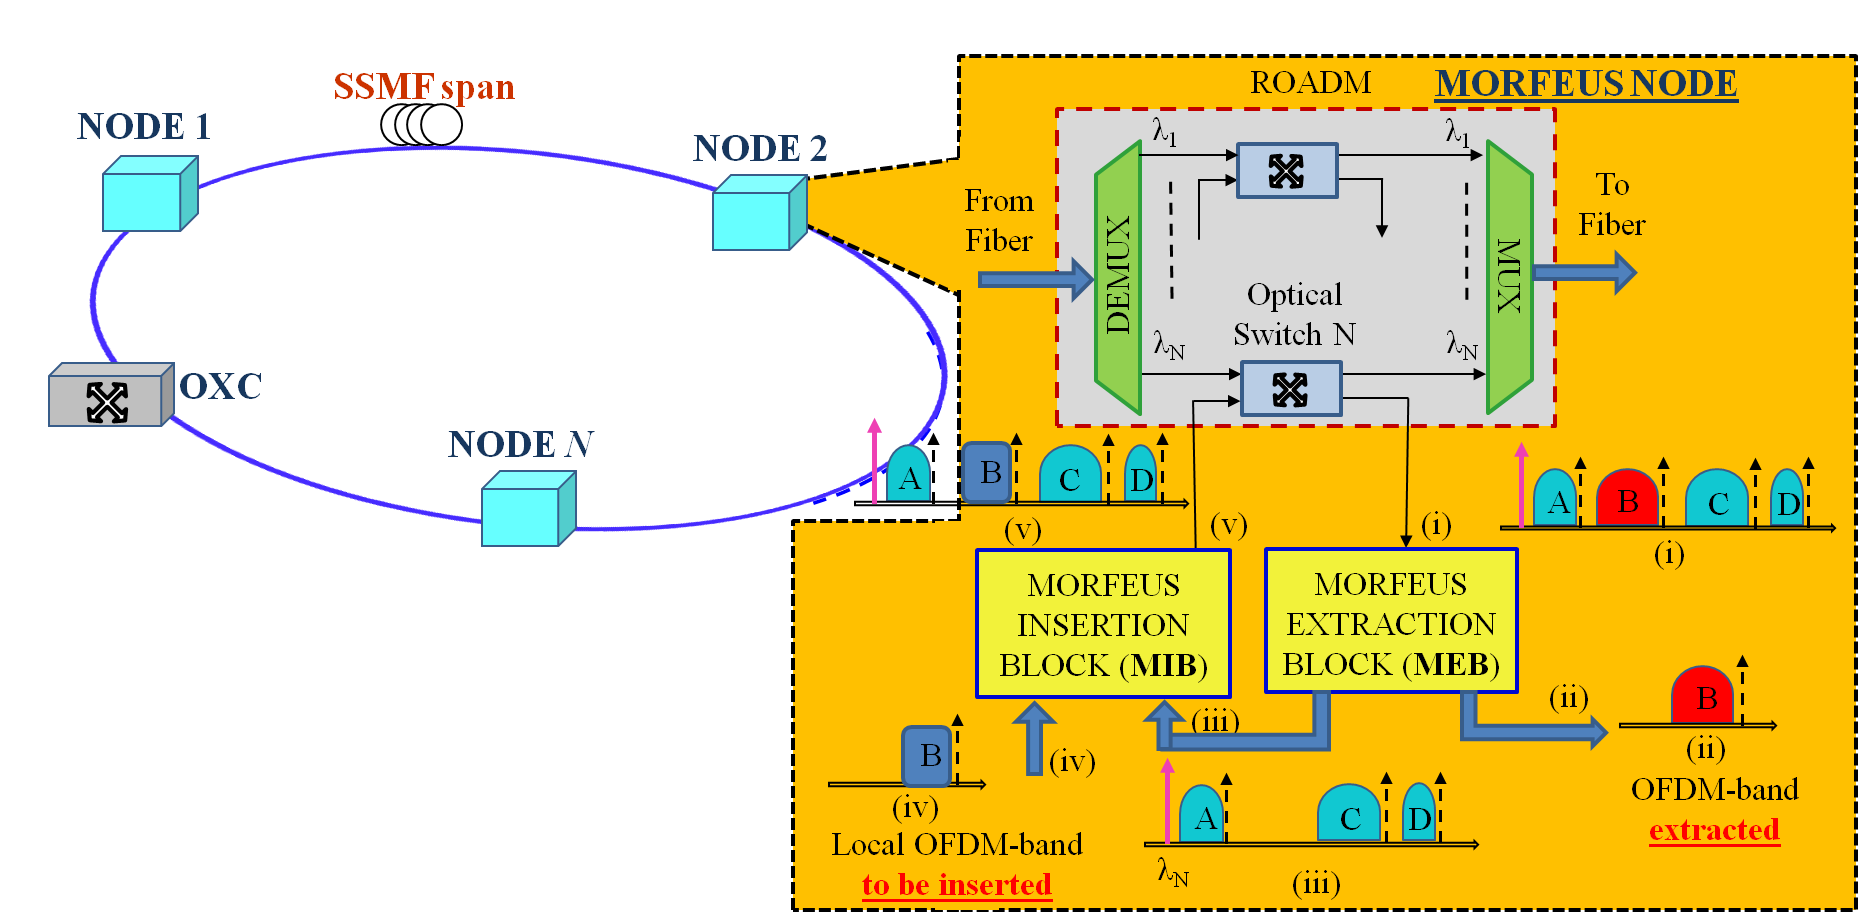
\includegraphics[width=0.45\textwidth]{NodeArchitecture2.png}
\caption{The MORFEUS network node structural architecture. DEMUX stands for wavelength demultiplexer and MUX stands for wavelength multiplexer.}
\label{morpheus_arch_node}
\end{figure}

In the figure \ref{morpheus_arch_node} we can see the structural architecture of a MORPHEUS network node. Each MORPHEUS node is essentially composed by two components sets. In one set we have the wavelengths MUX and DEMUX. This set has the task of catch by optical filtering or pass through a WDM signal depending of the network traffic demand. The other set treats a captured WDM signal as an OFDM signal and process it in the extraction and insertion band components here called MIB's(MORPHEUS Insertion Blocks) and MEB's(MORPHEUS Extraction Blocks) respectively.

\subsection{Proposed Algorithm}

Este estudo é proposto duas formas diferentes de implementar a heuristica LCL para o problema RWBA levando em consideração as diferentes formas de configuração.

\textcolor{red}{In this study we proposed a new strategy approach for band and wavelength assignment stages in the RWBA algorithm. Furthermore we compared the new approach with the strategies presented in \cite{imoc_2015}.
highlighted Extremes, a band assignment strategy that explores the extremes of spectrum to avoid its fragmentation. The new proposed strategy, that we called \textit{Least Capacity Loss} (LCL), is an efficient algorithm that we adapted from \cite{raul_lcl}. This algorithm was proposed firstly for the RSA problem. This strategy quantify the spare of bands for future requests. In this study we adapted the LCL algorithm to the RWAB context and proposed it as a new strategy for band and wavelength assignment as an undivided stage of RWBA algorithm.}

Let us define the capacity of a network as proportional to the number of ways of assigning a n-request. Once given a chosen route, the LCL algorithm have to choose an wavelength and a subset of bands that minimize the loss of number of ways of assignment for future requests. Assuming that each fiber of MORPHEUS network is composed by W wavelengths (indexed as 1, 2, ..., W ) and each wavelength $w \in W$ has B bands (indexed as 1, 2, ..., B).

\subsubsection{Subsubsection Heading Here}

\section{Results}

\subsection{Simulations and discussion}

\subsection{Impact of wavelength and band assignment algorithms on the network performance}

\section{Conclusion}
The conclusion goes here.

\appendices

\section*{Acknowledgment}

\ifCLASSOPTIONcaptionsoff
  \newpage
\fi



\begin{thebibliography}{1}

\bibitem{IEEEhowto:kopka}
H.~Kopka and P.~W. Daly, \emph{A Guide to \LaTeX}, 3rd~ed.\hskip 1em plus
  0.5em minus 0.4em\relax Harlow, England: Addison-Wesley, 1999.

\end{thebibliography}

\begin{IEEEbiography}{Michael Shell}
Biography text here.
\end{IEEEbiography}

\begin{IEEEbiographynophoto}{John Doe}
Biography text here.
\end{IEEEbiographynophoto}

\begin{IEEEbiographynophoto}{Jane Doe}
Biography text here.
\end{IEEEbiographynophoto}

\end{document}


